\section{Проектирование программного средства}
\label{sec:arch}

\subsection{Архитектура ПС}
\label{sec:arch_arch}

При проектировании архитектуры програмного средства я иходил из следующих побуждений:
\begin{itemize}
	\item обработка изображений требует хорошей производительности компьютера;
	\item у оператора должна быть возможность управлять процессом пропуска;
	\item програмное средство должно быть легко расширяемо с точки зрения изменения оработчика результатов распознанного номера;
	\item процесс обработки изображения представляет из себя последовательное выполенения сложных операций;
\end{itemize}

Для предоставления программе хороших вычислительных мощностей можно поместить её на мощьных сервер а клиенту лишь посылать результаты выполенения. Напрашивается вывод что для приложения лучше использовать клиент-серверную архитектуру. 

\begin{figure}[ht] 
    \centering
    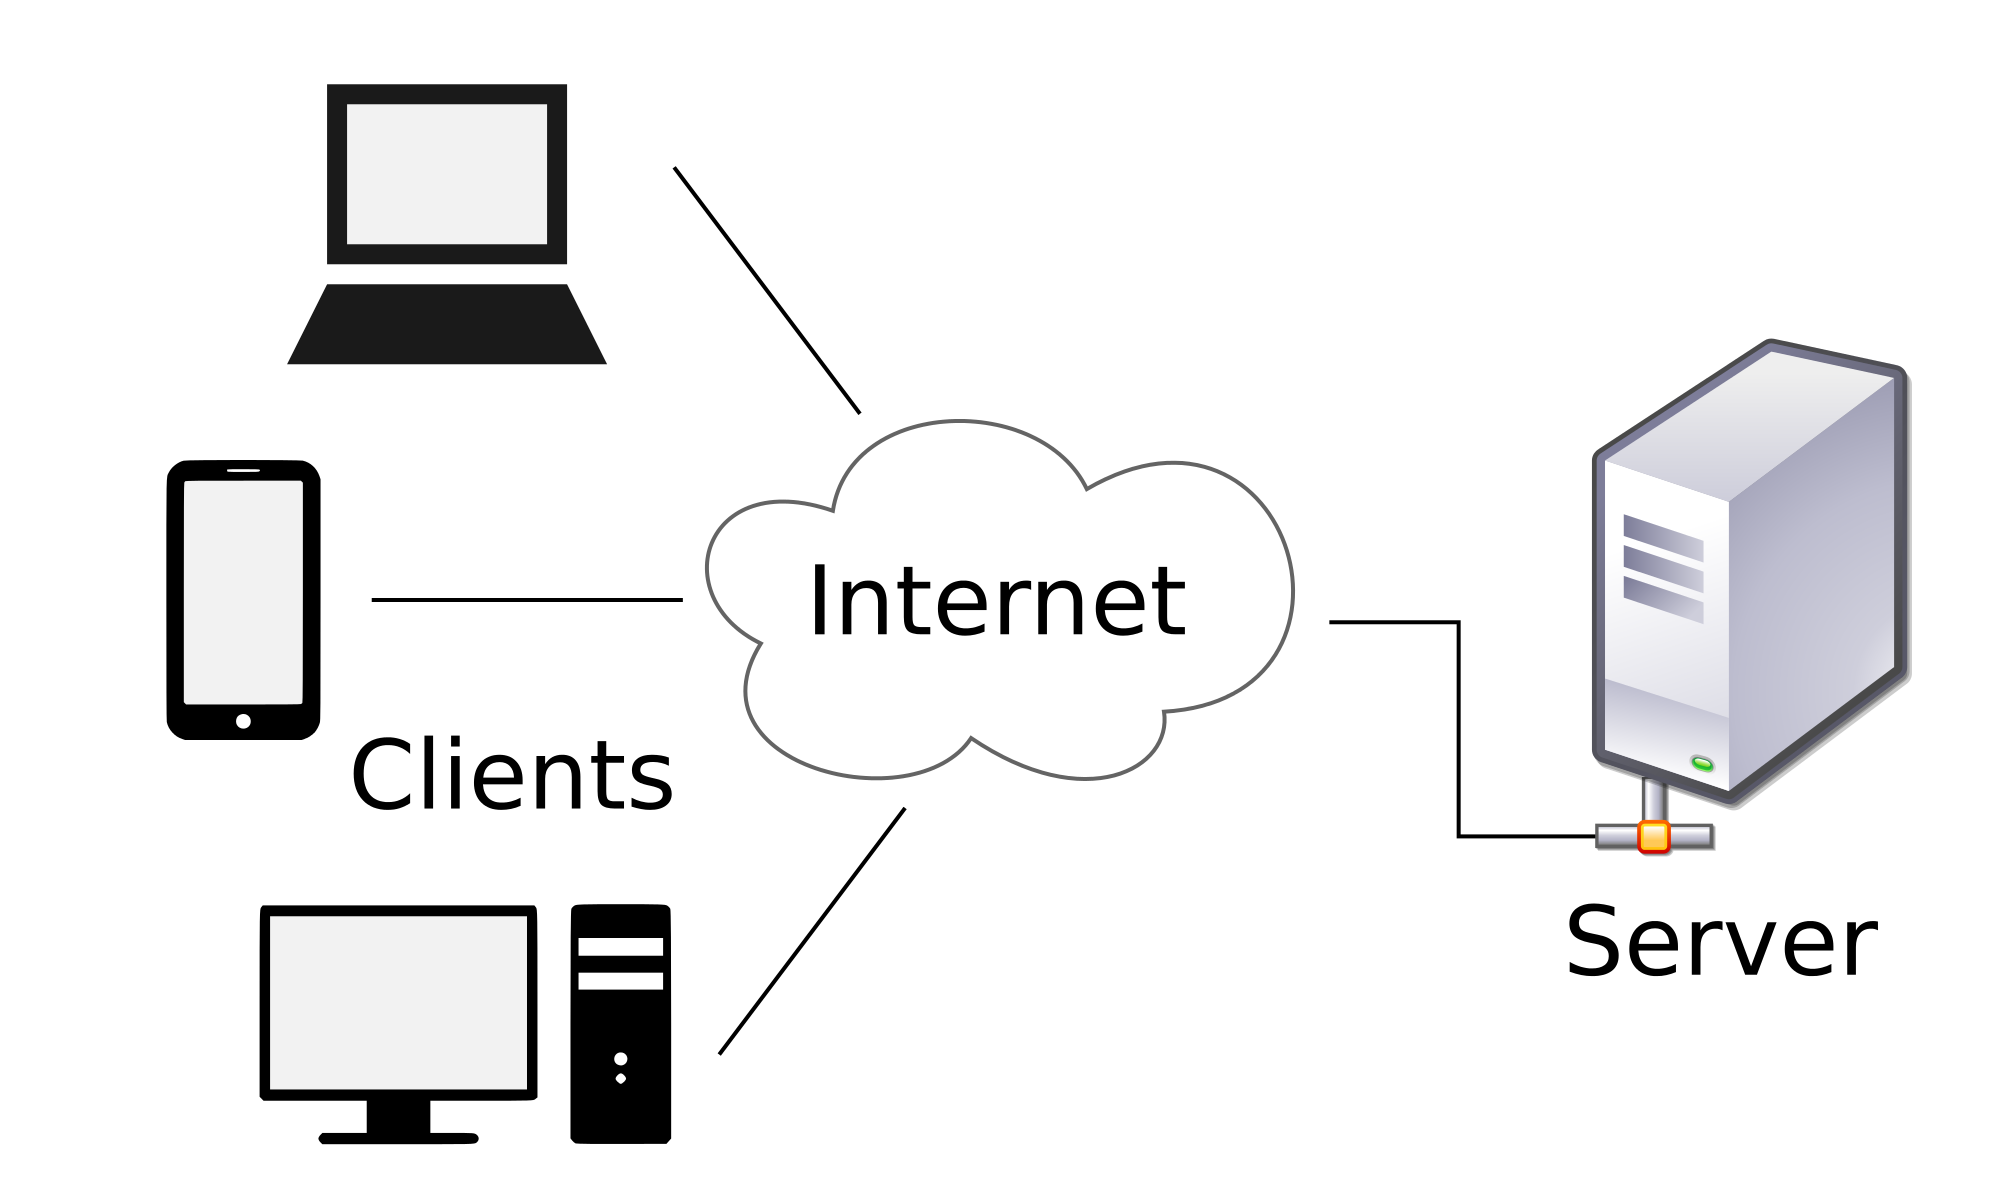
\includegraphics[scale=0.2]{Client-server-model.png}  
    \caption{Наглядная схема работы клиент-серверного приложения}
    \label{fig:arch_arch:client_server}
\end{figure}

Клиент-сервер - вычислительная или сетевая архитектура, в которой задания или сетевая нагрузка распределены между поставщиками услуг, называемыми серверами, и заказчиками услуг, называемыми клиентами. Физически клиент и сервер — это программное обеспечение. Обычно они взаимодействуют через компьютерную сеть посредством сетевых протоколов и находятся на разных вычислительных машинах, но могут выполняться также и на одной машине. Программы - сервера, ожидают от клиентских программ запросы и предоставляют им свои ресурсы в виде данных

Так же клиентскую часть лучше всего реализовать с помощью технологий html/css/java script. Это позволит использовать приложения практически с любого клиентского оборудование включая планшеты, компьютеры и телефоны. Общую схему работы приложения можно увидеть на рисунке \ref{fig:arch_arch:client_server}

Рассмотрим топологию нашего програмного средства представленного на рисунке \ref{fig:arch_arch:deployment}.
\begin{figure}[ht] 
    \centering
    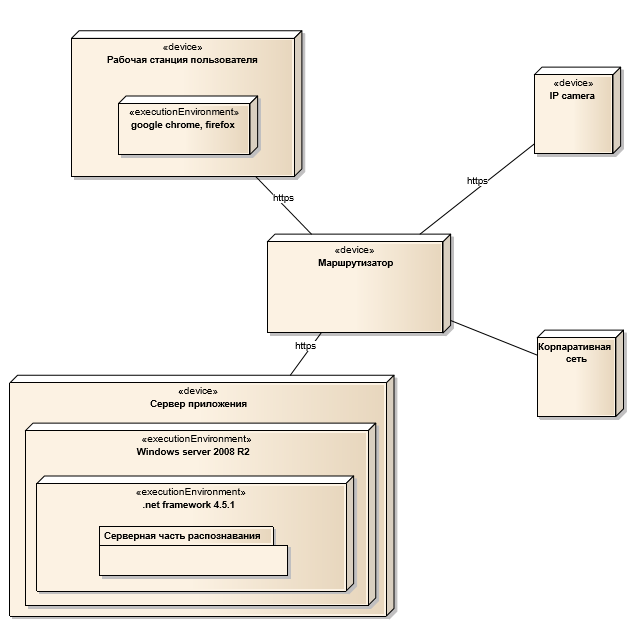
\includegraphics[scale=0.8]{deployment.png}  
    \caption{Диаграмма развертывания}
    \label{fig:arch_arch:deployment}
\end{figure}
Код отвечающий за обработку видеопотока будет выполняться на сервере, видеопоток он будет получать от IP камера расположенной в той же сети, результаты работы буду отпображаться пользователю на веб интерфейсе. В свою очередь пользовательский интерфейс тоже будет по сети подключаться к IP камере для трансляции текущей обстановки.

Процесс обработки изображений представляет из себя последовательно применение различных алгоритмов для исходного изображения. Конкретно эту часть лучше всего сделать используя архитектуру "Каналы и фильтры". Этот вид архитектуры подходит в том случае, если процесс работы приложения распадается на несколько шагов, которые могут выполнятся отдельными обработчиками. Основными компонентами являются "фильтр" и "канал". Иногда дополнительно выделяют "источник данных" и "потребитель данных". Применительно к разрабатываемому программному продукту, фильтр это конкретный алгоритм обрабатывающие изображение, источник данных - это видео поток от IP камеры, потребителем данных будут явятся плагины.

\begin{figure}[ht] 
    \centering
    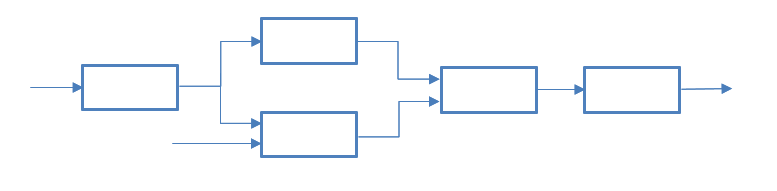
\includegraphics[scale=0.8]{pipes_and_filters.png}  
    \caption{Каналы и фильтры}
    \label{fig:arch_arch:pipes_and_filters}
\end{figure}

Каждый поток обработки данных – это серия чередующихся фильтров и каналов, начинающаяся источником данных и заканчивающаяся их потребителем. Каналы обеспечивают передачу данных и синхронизацию. Фильтр же принимает на вход данные и обрабатывает их, трансформируя в некое иное представление, а затем передает дальше.

Архитектура фильтров позволяет добится хорошо читаемого кода потому как реализует один из самых сложных принципов SOLID: принцип единственной обязанности, заключающийся в том что класс должен иметь только одну ответственность, то есть повлиять на спецификацию класса должно быть способно только одно потенциальное изменение в спецификации ПО. 

Как было отмеченно в разделе \ref{sub:domain:analogs} главный минус существующих систем это проблемная интеграция с существующими сервисами, конечно многие из них умеют работать с базами данных либо просто с файлами, но есть огромное количество сценариев итерации: отправить смс или email сообщение при распознанном номере, самостоятельно сделать запрос в стороннюю бд или отправить http запрос на шлагбаум и это только некоторые из них. Типичное решение такой проблемы поставить продукт с базовым функционалом в нашем случае это распознавание номеров и сделать его расширяемым с помощью плагинов. Это решение называется микроядерная архитектура. 

\begin{figure}[ht] 
    \centering
    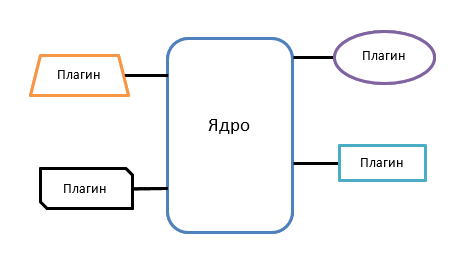
\includegraphics[scale=0.8]{plugins.png}  
    \caption{Микроядерная архитектура}
    \label{fig:arch_arch:plugins}
\end{figure}

Паттерн состоит из двух компонентов: основной системы (ядра) и плагинов. Ядро содержит минимум бизнес-логики, но руководит загрузкой, выгрузкой и запуском необходимых плагинов. Таким образом, плагины оказываются несвязанными друг с другом.

Поскольку плагины могут разрабатываться независимо друг от друга, такие системы обладают очень высокой гибкостью и, как следствие, легко тестируются. Производительность приложения, построенного на основе такой архитектуры, напрямую зависит от количества подключенных и активных модулей.

Если же взглянуть на архитектуру не только приложения но и все системы предприятия то мы увидим много сервисов выполняющих конкретно поставленную перед ними задачу, написанных на разных языках программирования с использованием разных платформ, и общающихся друг с другом по средствам сети. Этот подход называется микросервисная архитектура. В этом случае приложение разбивается на множество небольших сервисов, называемых микросервисами. Каждый микросервис включает в себя бизнес-логику и представляет собой совершенно независимый компонент. Сервисы одной системы могут быть написаны на различных языках программирования и общаться друг с другом, используя различные протоколы.

Поскольку каждый микросервис является отдельным проектом, вы можете распределить работу над ними между командами разработчиков, то есть над системой могут одновременно трудиться несколько десятков программистов. Микросервисная архитектура позволяет с легкостью масштабировать приложение - если вам понадобилось внедрить новую функцию (развертывать каждый микросервис можно по отдельности), просто напишите новый сервис, а если какой-то функцией никто не пользуется - отключите сервис.

Итого у нас получается клинт-серверное приложение, где на серверной части обработка изображения сделанна каналами и фильтрами, а обработка результатов представленна плагинами. В целом же наше приложения, смотря с уровня интеграции в корпоративную инфраструктуру, представляет из себя микросервис общающийся с другими микросервисами.

\subsection{Разработка  алгоритма ПС}
\label{sec:arch:algorythm}

Общий алгоритм распознавания номера можно увидеть на рисунке \ref{fig:arch:algorythm:image_processing_alg}, основывающийся на теоретическом анализе из \ref{sec:funcreq:teoretical_anolisys}.
\begin{figure}[ht] 
    \centering
    \includegraphics[scale=0.6]{image_processing.png}  
    \caption{Алгоритм распознавания номера}
    \label{fig:arch:algorythm:image_processing_alg}
\end{figure}
Судь алгоритма заключается в покадровой обработке видеопотока. На каждом карде он пытается найти автомобильный номер и распознать его. 
Сперва алгоритм находит автомобильный номер на картинке, если автомобильный номер не найден то компьютера приступает к обработке следующего кадра. Если же номер найден то на нем выделяются контуры, а затем происходит их анализ: анализируя размеры можно выделить символы среди прочих артефактов. Выделив символы их требуется вырезать и передать на распознавание. 
